\documentclass[hyperref={xetex}]{beamer}
\title{Wissenschaftliches Rechnen mit Matlab/Python}
\subtitle{Einheit 2 - Programmieren, Datenstrukturen}
\mode<article>
{
  \usepackage{fullpage}
  \usepackage{pgf}
  \usepackage{hyperref}
  \setjobnamebeamerversion{beamer}
}

\mode<presentation>
{
  %\usetheme{Frankfurt}
 %\usetheme{My}
  \usetheme{Madrid}
  % or ...
%\usecolortheme{seagull}
  %\setbeamercovered{transparent}
  %\setbeamercovered{dynamic}
  % or whatever (possibly just delete it)
}
\usenavigationsymbolstemplate{}
\usefonttheme{structurebold}
\usepackage{multimedia}
\usepackage{tikz}
\usepackage{fontspec,xunicode,xltxtra}
%\usepackage[scaled=.90]{helvet}
% Or whatever. Note that the encoding and the font should match. If T1
% does not look nice, try deleting the line with the fontenc.

\setbeamertemplate{footline}
{
\leavevmode
%\hbox{\begin{beamercolorbox}[wd=.5\paperwidth,ht=2.5ex,dp=1.125ex,
%leftskip=.3cm plus1fill,rightskip=.3cm]{author in head/foot}%
%    \usebeamerfont{author in head/foot}\insertshortauthor
%  \end{beamercolorbox}%
%  \begin{beamercolorbox}[wd=.5\paperwidth,ht=2.5ex,dp=1.125ex,leftskip=.3cm,
%rightskip=.3cm plus1fil]{title in head/foot}%
%    \usebeamerfont{title in head/foot}\insertshorttitle\hfill

\hfill\insertframenumber  \hspace{3pt}

%\inserttotalframenumber
%\hspace*{2ex}
%  \end{beamercolorbox}}%
  \vskip3pt%
}

%\usepackage[english]{babel}
\usepackage[ngerman]{babel}
\selectlanguage{ngerman}

%
% math/symbols
%
\usepackage{amssymb}
\usepackage{amsthm}
% \usepackage{latexsym}
\usepackage{amsmath}
%\usepackage{listings}
\usepackage[framed]{mcode}
%\usepackage{mcode}

\usepackage{mydef}
\usepackage{cmap} % you can search in the pdf for umlauts and ligatures
%\usepackage{colonequals} %corrects the definition-symbols \colonequals (besides others)
\title{Einführung in Matlab}
%
%\subtitle{Disputation} % (optional)

\author{Jochen Schulz}
% - Use the \inst{?} command only if the authors have different
%   affiliation.

\institute{Georg-August Universit\"at G\"ottingen \pgfimage[height=0.5cm]{../figures/unilogo3}}
% - Use the \inst command only if there are several affiliations.
% - Keep it simple, no one is interested in your street address.

\date{\today}

\subject{Einführung in Matlab}
% This is only inserted into the PDF information catalog. Can be left
% out. 



% If you have a file called "university-logo-filename.xxx", where xxx
% is a graphic format that can be processed by latex or pdflatex,
% resp., then you can add a logo as follows:

%\logo{\pgfimage[height=0.5cm]{figures/unilogo3}}


% Delete this, if you do not want the table of contents to pop up at
% the beginning of each subsection:
% \AtBeginSubsection[]
% {
%   \begin{frame}<beamer>
%     \frametitle{Aufbau}
%     \tableofcontents[currentsection,currentsubsection]
%   \end{frame}
% }

\AtBeginSection[]
{
  \begin{frame}<beamer>
    \frametitle{Aufbau}
    \tableofcontents[currentsection,currentsubsection]
  \end{frame}
}


\begin{document}



\begin{document}
\titlepage




\section{Programmieren}
%\item Aufgaben
 

\subsection{Schleifen}
%
% - Folie
%
\begin{frame}[fragile]{for - Schleife}
Wiederhole Befehle mit sich ändernder Indexvariable aus einem Indexsatz. 
\begin{matlabin}
for <indexvariable> = <Ausdruck>
  <Befehle>
end
\end{matlabin}
Ausdruck: \mcode{start:stepsize:end} oder Vektoren, Matrizen. 
\begin{pyin}
for <indexvariable> in <Liste>:
  <Befehle>
\end{pyin}
Liste: Liste oder Iterierbares Objekt mit beliebigen Inhalt.\\
Alternative: \textsl{List comprehensions} generieren Listen
  \begin{pyin}
[<Befehl> for <indexvariable> in <Liste> ]
\end{pyin}
\alert{Bemerkung:} 
\begin{itemize}
\item die Schleife geht alle Elemente der Liste oder des Ausdrucks durch, und führt die Befehle 
  darauf aus. 
\item \alert{Befehle} einrücken (Übersichtlichkeit; in Python Pflicht!) 
\end{itemize}

\end{frame}

%\textsl{Beispiel}:
% 
%\begin{pyin}
%[x**2 for x in range(4) if x % 2 == 0]
%\end{pyin}
%\begin{pyout}
%[0, 4]
%\end{pyout}


%
% - Folie
%
\begin{frame}[fragile]{Schleifen - Beispiele}
\begin{itemize}
\item Berechne $\sum_{i=1}^{1000} \frac{1}{i}$
\begin{matlabin}
sum=0; for j=1:1000, sum=sum+1/j; end, sum
\end{matlabin}
\begin{pyin}
sum([1/j for j in range(1,1000)])
\end{pyin}
\begin{matlab}
sum =  7.4855 
\end{matlab}
\item Berechnen dreier Werte
\begin{matlabin}
for x=[pi/6 pi/4 pi/3], sin(x), end
\end{matlabin}
\begin{pyin}
[sin(x) for x in [pi/6,pi/4,pi/3]]
\end{pyin}
\begin{matlab}
ans =    0.5000
ans =    0.7071
ans =    0.8660 
\end{matlab}
\end{itemize}
\end{frame}

\begin{frame}[fragile]{Schleifen - Beispiele II}
Matrix als {\it Ausdruck} bzw. als Schleifeniterator
\begin{matlabin}
for x=eye(3),  x' ,end
\end{matlabin}
\begin{matlab}
ans =     1     0     0
ans =     0     1     0
ans =     0     0     1 
\end{matlab}
\begin{pyin}
for x in eye(3,3): print x;
\end{pyin}
\begin{pyout}
  [ 1.  0.  0.]
  [ 0.  1.  0.]
  [ 0.  0.  1.]
\end{pyout}
\end{frame}


%
% - Folie
%
\begin{frame}[fragile]{Fixpunkt}
Suche ein $x_f \in \mathbb{R}$ so dass
\[ x_f = \cos (x_f ) \]
\begin{center}
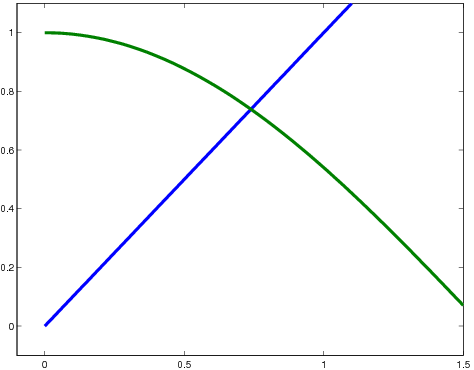
\includegraphics[height=5cm]{figures/fixpunkt}
\end{center}
Voraussetzung: Abbildung kontrahierend 
\[
\abs{f(x)-f(y)} \leq C \abs{x-y},\, C < 1\,  \forall  x,y \in  I
\]
% offenes Intervall I

\end{frame}
%
% - Folie
%
\begin{frame}[fragile]{Fixpunkt-Iteration}
Fixpunkt-Iteration 
\[ x_{k+1}=cos(x_k) \]
bei geeignetem Startwert $x_0$.  \\
\centering{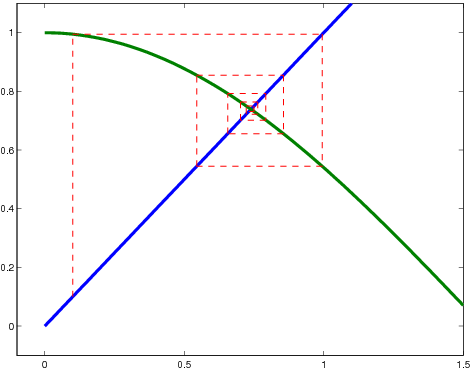
\includegraphics[height=5cm]{figures/fixpunkt1}}\\
(Funktioniert wenn die Abbildung kontrahierend ist)
\end{frame}

%
% - Folie
%
\begin{frame}[fragile]{Matlab: Fixpunkt-Iteration}
\begin{matlabin}
% Plot 1
x = linspace(0,1.5,50);
y = cos(x);
plot(x,x,x,y,'LineWidth',3);
axis([-0.1 1.5 -0.1 1.1]);
hold on;
pause; % stoppt bis eine Taste gedrückt wird
z(1) = 0.1; % Anfangswert
it_max = 10; % Iterationsschritte 
for i = 1:it_max
    z(i+1) = cos(z(i));
    plot([z(i) z(i)], [z(i) z(i+1)],'r--','LineWidth',1);
    pause;
    plot([z(i) z(i+1)],[z(i+1) z(i+1)],'r--','LineWidth',1);
    hold on;
    pause; % stoppt bis eine Taste gedrückt wird
end;
\end{matlabin}
\end{frame}

\begin{frame}[fragile]{Python: Fixpunkt-Iteration}
  \begin{pyin}
x = linspace(0,1.5,50)
y = cos(x)
plot(x,x,x,y,linewidth=3)
z = [] # Leere Liste initialisieren
z.append(0.1) # Anfangswert
it_max = 10 # Iterationsschritte 
for i in arange(0,it_max):
    z.append( cos(z[i]) )   
    plot([z[i], z[i]], [z[i], z[i+1]],'r--',linewidth=1)
    plot([z[i], z[i+1]],[z[i+1], z[i+1]],'r--',linewidth=1)    
  \end{pyin}
\end{frame}
%
% - Folie
%
\begin{frame}[fragile]{Einige Grafikbefehle}
\begin{itemize}
\item \alert{ \mcode{figure()}} \\
startet ein Grafik-Fenster.
\item \alert{ \mcode{hold on}}\\
 alle Grafiken in einem Fenstier werden \"ubereinander gezeichnet. (Python: default!)
\item \alert{ \mcode{hold off}} (Default)\\
 bestehende Grafik wird gel\"oscht und durch die neue Grafik ersetzt. (Python: jeweils neue figures erzeugen)
\end{itemize}
\end{frame}
\begin{frame}[fragile]{Vandermonde-Matrix I}
Berechne zu einem gegebenen Vektor
  $x=(x_1, \dots ,x_n)$ die Vandermonde-Matrix
{ \[ V:= \left(\begin{array}{ccccc} 
1 & x_1 & x_1^2 & \hdots & x_1^{n-1}\\
1 & x_2 & x_2^2 & \hdots & x_2^{n-1}\\
\vdots & \vdots & \vdots & \vdots & \vdots\\
1 & x_n & x_n^2 & \hdots & x_n^{n-1}\\
\end{array} \right).  \]}
\end{frame}
%
%
%
\begin{frame}[fragile]{}
  \begin{matlabin}
function V = vandermonde2(x)
  n = length(x);
  V = zeros(n,n);
  for i = 1:n
    for j = 1:n
      V(i,j) = x(i)^(n-j);
    end
  end
  \end{matlabin}
  \begin{pyin}
def vandermonde2(x):
  n = len(x)
  V = zeros((n,n))
  for i in arange(0,n):
    for j in arange(0,n):
      V[i,j] = x[i]**(n-j-1)
  return V
  \end{pyin}
\end{frame}



\subsection{Bedingungen}
%
%
%
\begin{frame}[fragile]{Bedingung}
\begin{columns}[t,onlytextwidth]
 \column{0.45\textwidth}
Matlab
\begin{matlabin}
if  <Ausdruck>
   <Befehle>
elseif <Ausdruck>
  <Befehle>
else
   <Befehle>
end
\end{matlabin}
 \column{0.45\textwidth}
Python
\begin{pyin}
if <Ausdruck>:
  <Befehle>
elif <Ausdruck>:
  <Befehle>
else:
  <Befehle>
\end{pyin}
\end{columns}
  \begin{pyin}
[<Befehl> for <indexvariable> in <Liste> if <ausdruck>]
\end{pyin}

Die Befehle zwischen \mcode{if} und \mcode{end} (bzw. nach : und bis Ende Einrückung) werden ausgeführt, wenn
der \textit{Ausdruck} wahr (\isage{True}) ist.\\
Sonst werden die \mcode{elseif}-Bedingungen geprüft, und falls keine dieser wahr ist, wird (soweit vorhanden) der \mcode{else}-Block ausgeführt.

\alert{Hinweis}: \textit{Ausdruck} ist wahr, wenn   alle Einträge von \textit{Ausdruck} ungleich $0$ sind.
\end{frame}
%
%
%
\begin{frame}[fragile]{Quadratische Gleichung}
\alert{ \[  \left\{ \begin{array}{l} \mbox{Suche }  x \in \mathbb{R},
 \mbox{ so dass } \\
 x^2+px +q =0  \end{array} \right. \]}
Fallunterscheidung für $d:=\frac{p^2}{4} -q$:
\begin{description}
\item [Fall a)]: \alert{ $d>0$} \quad 2 Lösungen: $x=-\frac{p}{2} \pm \sqrt{d}$ \\
\item [Fall b)]: \alert{ $d=0$} \quad 1 Lösung: $x=-\frac{p}{2}$\\
\item [Fall c)]: \alert{ $d<0$} \quad keine Lösung
\end{description}
\end{frame} 
%
%
%
\begin{frame}[fragile]{Matlab: Implementierung}
\begin{matlabin}
function [anz_loesungen, loesungen]=quad_gl(p,q)
d=p^2/4-q; % Diskriminante
% 2 Loesungen
if d>0 
    anz_loesungen=2;
    loesungen=[-p/2-sqrt(d) -p/2+sqrt(d)];
end
% 1 Loesung
if d==0 
    anz_loesungen=1;
    loesungen=[-p/2];
end
% 0 Loesungen
if d<0 
    anz_loesungen=0;
    loesungen=[];
end
\end{matlabin}
\end{frame}
%
%
%
\begin{frame}[fragile]{Python: Implementierung}
\begin{pyin}
def quad_gl(p,q):
    d = p**2/4-q # Diskriminante
    # 2 Loesungen
    if d>0:
        anz_loesungen=2
        loesungen=array([-p/2-sqrt(d), -p/2+sqrt(d)])
    # 1 Loesung
    if d==0:
        anz_loesungen=1
        loesungen=array([-p/2])
    # 0 Loesungen
    if d<0:
        anz_loesungen=0
        loesungen=array([])
    return anz_loesungen, loesungen
\end{pyin}
\end{frame}

%
%
%
\begin{frame}[fragile]{Logische Operationen}
\begin{itemize}
\item logische Variablen (Datentyp ist \alert{logical}(Matlab) \alert{bool}(Python). 
\item Variablen dieses Typs sind entweder \mcode{true} (1) oder
  \mcode{false} (0) (Python: \isage{True} oder \isage{False})
\item Matlab: Numerische Werte ungleich $0$ werden als \mcode{true} gewertet.
\end{itemize}
\begin{matlabin}
a = (1<2)
\end{matlabin}
\begin{matlab}
a = 1 
\end{matlab}
\begin{matlabin}
b = ([ 1 2 3 ] < [ 2 2 2 ]) 
\end{matlabin}
\begin{matlab}
b =   1     0     0 
\end{matlab}
\begin{matlabin}
whos 
\end{matlabin}
\begin{matlab}
  Name Size Bytes  Class
  a     1x1  1  logical array
  b     1x3  3  logical array 
\end{matlab}
\end{frame}
%
%
%
\begin{frame}[fragile]{Vergleichs-Operatoren}
\begin{matlabin} 
a=[1 1 1], b=[0 1 2] 
\end{matlabin}
\begin{center}
\begin{tabular}{cll}
Operation & Bedeutung & Ergebnis\\
\hline
\mcode{a ==  b} & gleich &   \mcode{0     1     0}\\
\mcode{a \~= b} & ungleich & \mcode{1     0     1}\\
\mcode{a < b} & kleiner & \mcode{0     0     1}\\
\mcode{a > b} & größer & \mcode{1     0     0}\\
\mcode{a <= b} & kleiner oder gleich & \mcode{0     1     1}\\
\mcode{a >= b} & größer oder gleich & \mcode{1     1     0}\\
\end{tabular}
\end{center}
\alert{Bem:} \alert{ 1 = wahre Aussage, 0 = falsche Aussage}\\
\alert{Bem:} Komponentenweise Vergleiche sind auch für Matrizen
gleicher Größe möglich! 
\end{frame}
%
%
%
\begin{frame}[fragile]{Logische Operatoren}
\begin{center}
\begin{tabular}{|c|l||c|l|}
\hline
\mcode{\&}(Ma) \mcode{and}(Py) & logisches und & \mcode{\~}(Ma) \mcode{!}(Py)& logisches nicht \\
\mcode{|}(Ma) \mcode{or}(Py) & logisches oder & \mcode{xor}(Ma) & exklusives oder\\
\hline
\end{tabular}
\end{center}
Beispiele:\\
\begin{matlabin} 
x=[-1 1 1]; y=[1 2 -3];
\end{matlabin}
\vspace*{0.5cm}
\begin{minipage}{5cm}
\begin{matlabin}
>> (x>0) & (y>0)
ans =
     0     1     0
\end{matlabin}
\vspace*{0.5cm}
\begin{matlabin}
>> (x>0) | (y>0)
ans =
     1     1     1
\end{matlabin}
\end{minipage} \hfill
\begin{minipage}{5cm}
\begin{matlabin}
>> ~( (x>0) & (y>0))
ans =
     1     0     1
\end{matlabin}
\vspace*{0.5cm}
\begin{matlabin}
>> xor(x>0,y>0)
ans =
     1     0     1
\end{matlabin}
\end{minipage}
\end{frame}
%for k in [1..3]:
%    if k>1:
%            k
%            x = 2; y = 2
%            for k in [1..4]:
%              x = x+k
%                y = y^k
%                        print (``x ist {0} und y ist {1}''.format(x,y))
%                        x,y
%
%
%
\begin{frame}[fragile]{While-Schleifen}
\begin{matlabin}
while <Ausdruck>
  <Befehle>
end
\end{matlabin}
\begin{pyin}
while <Ausdruck>:
  <Befehle>
\end{pyin}
Die Befehle werden wiederholt,  so lange die Bedingung {\it Ausdruck}
wahr ist.  \\

\textbf{Beispiel:} Berechne \alert{ $\sum_{i=1}^{1000} \frac{1}{i}$}.
\begin{matlabin}
n = 1000; sum = 0; i = 1; 
while (i <= n) 
  sum = sum+(1/i); 
  i = i+1;  
end
\end{matlabin}
\begin{pyin}
n = 1000; sum = 0; i = 1;
while (i <= n):
  sum += 1./i
  i += 1
\end{pyin}

\end{frame}
%
%
%
\begin{frame}[fragile]{Größter gemeins. Teiler (ggT)}
Berechnung des ggT von natürlichen Zahlen $a$ und $b$ mit Hilfe des
euklidischen Algorithmus\\[1cm]

\alert{Idee:} Es gilt \alert{ $ggT(a,b)=ggT(a,b-a)$} für $a<b$.\\[1cm]

\begin{block}{Algorithmus}
Wiederhole,  bis $a=b$
\begin{itemize}
\item Ist $a>b$, so $a=a-b$.
\item Ist $a<b$, so $b=b-a$ 
\end{itemize}
\end{block}
\end{frame}

\begin{frame}[fragile]{Implementierung}
\begin{matlabin}
function a = ggt(a,b)
while (a ~= b)
  if (a > b)
    a = a-b;
  else
    b = b-a;
  end
end
\end{matlabin}
\begin{pyin}
def ggt(a,b):
  while (a != b):
    if (a > b):
      a -= b
    else:
      b -= a
  return a
\end{pyin}
\end{frame}
%
%
%
\begin{frame}[fragile]{\textit{break}}
\begin{itemize}
\item  Der Befehl \mcode{break} verläßt die \mcode{while} oder
  \mcode{for}-Schleife.
\begin{matlabin}
x=1;
while 1
  xmin=x;
  x=x/2;
  if x==0
    break
  end
end
xmin
\end{matlabin}
\begin{matlab}
xmin = 4.9407e-324
\end{matlab} 

\end{itemize}
\end{frame}

\begin{frame}[fragile]{\textit{continue}}
\begin{itemize}
 \item  Durch \mcode{continue} springt man sofort in die
  nächste Iteration der Schleife, ohne die restlichen Befehle zu
  durchlaufen.
\begin{matlabin}
for i=1:10
  if i<5
    continue
  end
  x(i)=i;
end
x
\end{matlabin}
\begin{matlab}
x =  0  0  0  0  5  6  7  8  9  10
\end{matlab}
 
\end{itemize}
\end{frame}



\subsection{Allgemeines}
%
% Folie
%
\begin{frame}[fragile]{Operator Rangfolge}
\begin{tabular}{|cp{10cm}|}
\hline
Level & Operator\\
\hline
1 & Exponent (\mcode{^}, \mcode{.^}), \mcode{transpose}\\
2 & logische Verneinung (\mcode{\~},\mcode{!})\\
3 & Multiplikation (*,.*), Division (\mcode{/},\mcode{./},\mcode{\\}, \mcode{.\\})\\
4 & Addition (+), Subtraktion (-)\\
5 & Doppelpunktoperator (:)\\
6 & Vergleichsoperatoren (\mcode{<},\mcode{>},\mcode{<=},\mcode{>=},\mcode{==},\mcode{\~=},\mcode{!=})\\ 
7 & Logisches und (\mcode{\&}, \mcode{and})\\
8 & Logisches oder (\mcode{|}, \mcode{or})\\
\hline
\end{tabular}\\[0.5cm]
{\scriptsize Bei gleicher Rangfolge wird von links nach rechts ausgewertet. \\
Die Rangfolge kann durch Klammersetzung geändert werden.}

\end{frame}


%
% Slide
%
%\begin{frame}[fragile]{Warnung}
%\begin{center}
%\alert{ Wiederholte Anwendung von Script-Files kann zu Fehlern führen!}\\[0.5cm]
%\end{center}
%\begin{columns}[t]
% \column{0.4\textwidth}
%\alert{Programm}
%\begin{matlabin}[basicstyle=\scriptsize]
%% plotte_sin.m
%
%disp(['Plot der Sinus'...
%  'Funktion auf [0,10]']);
%n = input(['Plot an '...
%   'wievielen Punkten?']);
%x = linspace(0,10,n);
%for i=1:n
%y(i) = sin(x(i));
%end; 
%plot(x,y);
%\end{matlabin}
%\column{0.5\textwidth}
%\alert{ Aufruf}
%\begin{matlabin}[basicstyle=\scriptsize]
%>> plotte_sin
%Plot der Sinus Funktion auf [0,10]
%Plot an wievielen Punkten?20
%>> plotte_sin
%Plot der Sinus Funktion auf [0,10]
%Plot an wievielen Punkten?10
%??? Error using ==> plot
%Vectors must be the same lengths.
%
%Error in ==> plotte_sin.m
%On line 9  ==> plot(x,y);
%\end{matlabin}
%\end{columns}
%\end{frame}
%
% Slide
%
%\begin{frame}[fragile]{Gültigkeitsbereich von Variablen}
%\begin{itemize}
%\item \alert{Variablen in Skript-Files} 
%\begin{itemize}
%\item globaler Workspace (d.h. bereits vorhandene Variablen können direkt benutzt oder
%  überschrieben werden)
%\item gültig bis explizit gelöscht
%\end{itemize}
%\item \alert{Variablen in Function-Files} 
%\begin{itemize}
%\item innerhalb der Funktion definiert und werden bei Verlassen der Funktion
%  gelöscht.
%\item Variablen des globalen Workspace können nicht benutzt werden (\alert{Vorsicht}: das funktioniert in Python leider schon, vermeidet es dennoch!)
%\end{itemize} 
%\end{itemize}
%\end{frame}
%
% Slide
%
\begin{frame}[fragile]{globale Variablen}
Mittels des Befehls \alert{ \mcode{global}} können Variablen des
globalen Workspace auch für Funktionen manipulierbar gemacht werden.
\bigskip
\begin{columns}[t]
 \column{0.45\textwidth}
\alert{ Funktion}
\begin{matlabin}
function f=myfun(x)
% myfun.m
% f(x)=x^alpha sin(1/x)

global alpha
f=x.^alpha.*sin(1./x);
\end{matlabin}
 \column{0.45\textwidth}
\alert{ Plotten}
\begin{matlabin}
% plot_myfun
global alpha
alpha_w=[ 0.4 0. 6 1 1.5 2];
for i = 1:length(alpha_w)
    alpha = alpha_w(i);
    fplot(@myfun,[0.1,1])
    hold on;
end
hold off;
\end{matlabin}
\end{columns}
\end{frame}
%
% Slide
%
\begin{frame}[fragile]{Ein Guter Stil I }
\begin{itemize}
\item Beschreibung: Alle Programme/Funktionen sollten zu Beginn einen Kommentar enthalten, in
  dem beschrieben wird, was das Programm macht.
  \begin{itemize}
      \item Programmbeschreibung
      \item Eingabevariablen
      \item Ausgabevariablen
      \item Beispiele
  \end{itemize}
\item Vor und nach logischen Operatoren und $=$ sollte ein Leerzeichen
  gesetzt werden.
\item Man sollte pro Zeile nur einen Befehl verwenden.
\item Befehle in  Strukturen, wie  \mcode{if}, \mcode{for}
  oder \mcode{while}, sollten eingerückt werden (Python erzwingt dies sowieso)
%\item Variablen Namen für Matrizen sollten mit einem Großbuchstaben
 % beginnen. 
\end{itemize}
\end{frame}
%
% Slide
%
\begin{frame}[fragile]{Ein Guter Stil II}
\begin{itemize}
\item Die Namen der Variablen sollten, soweit möglich, selbsterklärend
  sein.
\item Verfasst man umfangreiche Programme, so sollten Funktionalitäten, die
  eine logische Einheit bilden in einen separaten Datei, Unterverzeichnis oder Modul gelegt werden.
\item Potenzielle Fehler sollten, soweit möglich, aufgefangen
  werden. Speziell sollten die Eingabeparameter der Funktionen
  geprüft werden. 
\end{itemize}
\end{frame}


\section{Datenstrukturen}
%
%
%
\begin{frame}[fragile]{Datentypen}
\begin{itemize}
\item \alert{Datentypen} werden bestimmt durch ihre Eigenschaften.
\item Zuweisung des Datentyps ist {\it implizit}. 
\item Operationen können Typen ändern.
\item Achtung: Daher ist nicht immer klar, welchen Typ eine Variablen gerade hat.
%\item Einzelne Elemente eines Datentyps werden \alert{Objekte} genannt. 
%\item Ein \alert{Objekt} besteht meist aus drei Teilen: \alert{Bezeichner}, \alert{Referenzen} 
%und \alert{Werte} des Objekts.  
%\item \alert{Variablen} sind Datenobjekte deren Werte w\"ahrend eines
%Programmablaufs ver\"andert werden k\"onnen. 
\end{itemize}
\end{frame}
%
%
%
%\begin{frame}[fragile]{Datentypen in MATLAB}
%\begin{itemize}
%\item Alle Variablen sind Felder (Array). Ein Skalar ist eine $1 \times
%1$-Matrix. 
%\item Den Datentyp eines Objekts $a$ kann durch den Befehl \mcode{class(a)} bestimmt werden.
%\end{itemize}
%\end{frame}
%
%
%
%\begin{frame}[fragile]{Datentypen in MATLAB}
%\begin{itemize}
%\item Gleitkommazahlen (Komplexe Zahlen)
%\item Characters und Strings
%\item Strukturen
%\item Cell Arrays
%\item Funktionen
%\item Sparse Matrizen
%\item Integer-Zahlen
%\item Logische Ausdr\"ucke
%\end{itemize}
%\end{frame}

\subsection{Zahlen}
%
% Folie
%
\begin{frame}[fragile]{Gleitkommazahlen / Maschinengenauigkeit}
\begin{itemize}
\item Standard-Datentyp ist ein Array von Gleitkommazahlen (\mcode{double}).
\item Abstand von $1$ zur nächsten Gleitkommazahl: $\epsilon
  = 2^{-52} \sim 2.2\cdot10^{-16}$ (\mcode{eps}(Matlab), \isage{spacing(1)}(Python))
\item Sei $x \in \mathbb{R}$ eine reelle Zahl und $\tilde x$ die
  Darstellung im Computer. Dann gilt für den Rundungsfehler \\[-0.5cm]
\[ \frac{|x - \tilde x|}{|x|}\leq \frac{1}{2} \epsilon .\]
\item größte bzw. kleinste darstellbare positive Zahl
\mcode{realmin}(Matlab) bzw. \mcode{realmax}(Matlab) und \isage{sys.float_info}(Python)
\end{itemize}
\end{frame}
%
% Folie
%
\begin{frame}[fragile]{Ausnahmen}
\begin{itemize}
\item Ist eine Zahl größer als \mcode{realmax}, so meldet MATLAB einen
  'Overflow' und gibt als Ergebnis \mcode{Inf} zurück.
\begin{matlabin}
realmax*1.1
\end{matlabin}
\begin{matlab}
 ans =   Inf
\end{matlab}

\item Bei Operationen wie $0/0$  oder $\infty / \infty$, erhält man als Ergebnis
  \mcode{NaN} ({\it Not a Number}).
\begin{matlabin}
0/0 
\end{matlabin}
\begin{matlab}
Warning: Divide by zero.
ans =   NaN 
\end{matlab}

\end{itemize}
\end{frame}
%
% Folie
%
\begin{frame}[fragile]{Umgang mit NaN und       Inf  }
  Matlab:
\begin{itemize}
\item \alert{ \mcode{isinf}} und \alert{ \mcode{isnan}} testen auf
$\infty$ bzw. NaN.
 \begin{matlabin}
isnan(0/0), isinf(1.2*realmax)
\end{matlabin}
\begin{matlab}
ans =   1  ans =   1
\end{matlab}
\end{itemize}
Python:
\begin{itemize}
  \item brauchen Modul \textsl{NumPy}\\
    \begin{pyin}
import numpy as np
    \end{pyin}
  \item \isage{np.isinf} und  \isage{np.isnan} testen auf
    $\infty$ bzw. NaN.
    \begin{pyin}
np.isinf(sys.float_info.max*1.1)      
    \end{pyin}
    \begin{pyout}
True      
    \end{pyout}
\end{itemize}

\end{frame}
%
% Folie
%
%\begin{frame}[fragile]{Single}
%\begin{itemize}
%\item \"Ahnlich wie in C gibt es den Datentyp \mcode{single}. Es ist eine
%Darstellung in geringerer Genauigkeit. 
%\item Durch den Befehl \alert{ \mcode{single()}} wird eine \mcode{double}-Zahl in
%eine \mcode{single}-Zahl konvertiert. 
%\item Arithmetische Operationen mit \mcode{double}- und \mcode{single}-Objekten
%ergeben  \mcode{single}-Objekte.
%\end{itemize}
%\end{frame}
%
% Folie
%
%\begin{frame}[fragile]{Single}
%\begin{matlabin}
%a = sqrt(2); b = single(a);
%c = a+b; d = a-b
%\end{matlabin}
%\begin{matlab}
%d =
%  2.4203e-08
%\end{matlab}
%\begin{matlabin}
%whos
%\end{matlabin}
%\begin{matlab}
%  Name   Size     Bytes  Class    
%  a      1x1        8  double              
%  b      1x1        4  single              
%  c      1x1        4  single              
%  d      1x1        4  single  
%\end{matlab}
%\begin{matlabin}
%[realmax, single(realmax)], realmax
%\end{matlabin}
%\begin{matlab}
%ans =
%   Inf   Inf
%ans =
%  1.7977e+308
%\end{matlab}
%\end{frame}

%
% Folie
%
%\begin{frame}[fragile]{Darstellungsformate am Beispiel $1/7$}
%\begin{tabular}{ll}
%\alert{ \mcode{format short}} &  0.1429 \\
%\alert{ \mcode{format short e} }& 1.4286e-01\\
%\alert{ \mcode{format short g} }&0.14286\\
%\alert{ \mcode{format long} }& 0.14285714285714\\
%\alert{ \mcode{format long g} }& 0.142857142857143\\
%\alert{ \mcode{format long e} }& 1.428571428571428e-01\\
%\end{tabular}
%
%Das Default-Format ist \mcode{short}. 
%\end{frame}


\begin{frame}[fragile]{Beispiel - Berechnung von $e$}
Approximation der Exponentialfunktion durch eine Taylor-Reihe
\begin{equation*}
 P_n(x) = \sum_{j=0}^n\frac{x^j}{j!} 
\end{equation*}

\begin{matlabin}
x = -10:0.01:10; % die x-Werte
expx = exp(x); % die wahre Exponentialfunktion
for n=0:1:25
    % so viele Nullen wie x Elemente hat
    sum=zeros(size(x));     
    for j=0:n
        % das berechnet die Partialsumme
        sum=sum+x.^j/factorial(j); 
    end
    % plottet relativen Fehler
    plot(x,(sum-expx)./expx); 
    % wir plotten alles uebereinander
    hold on 
end
\end{matlabin}

\end{frame}

\begin{frame}[fragile]{Berechnung von $e$ - Relativer Fehler}
\begin{center}
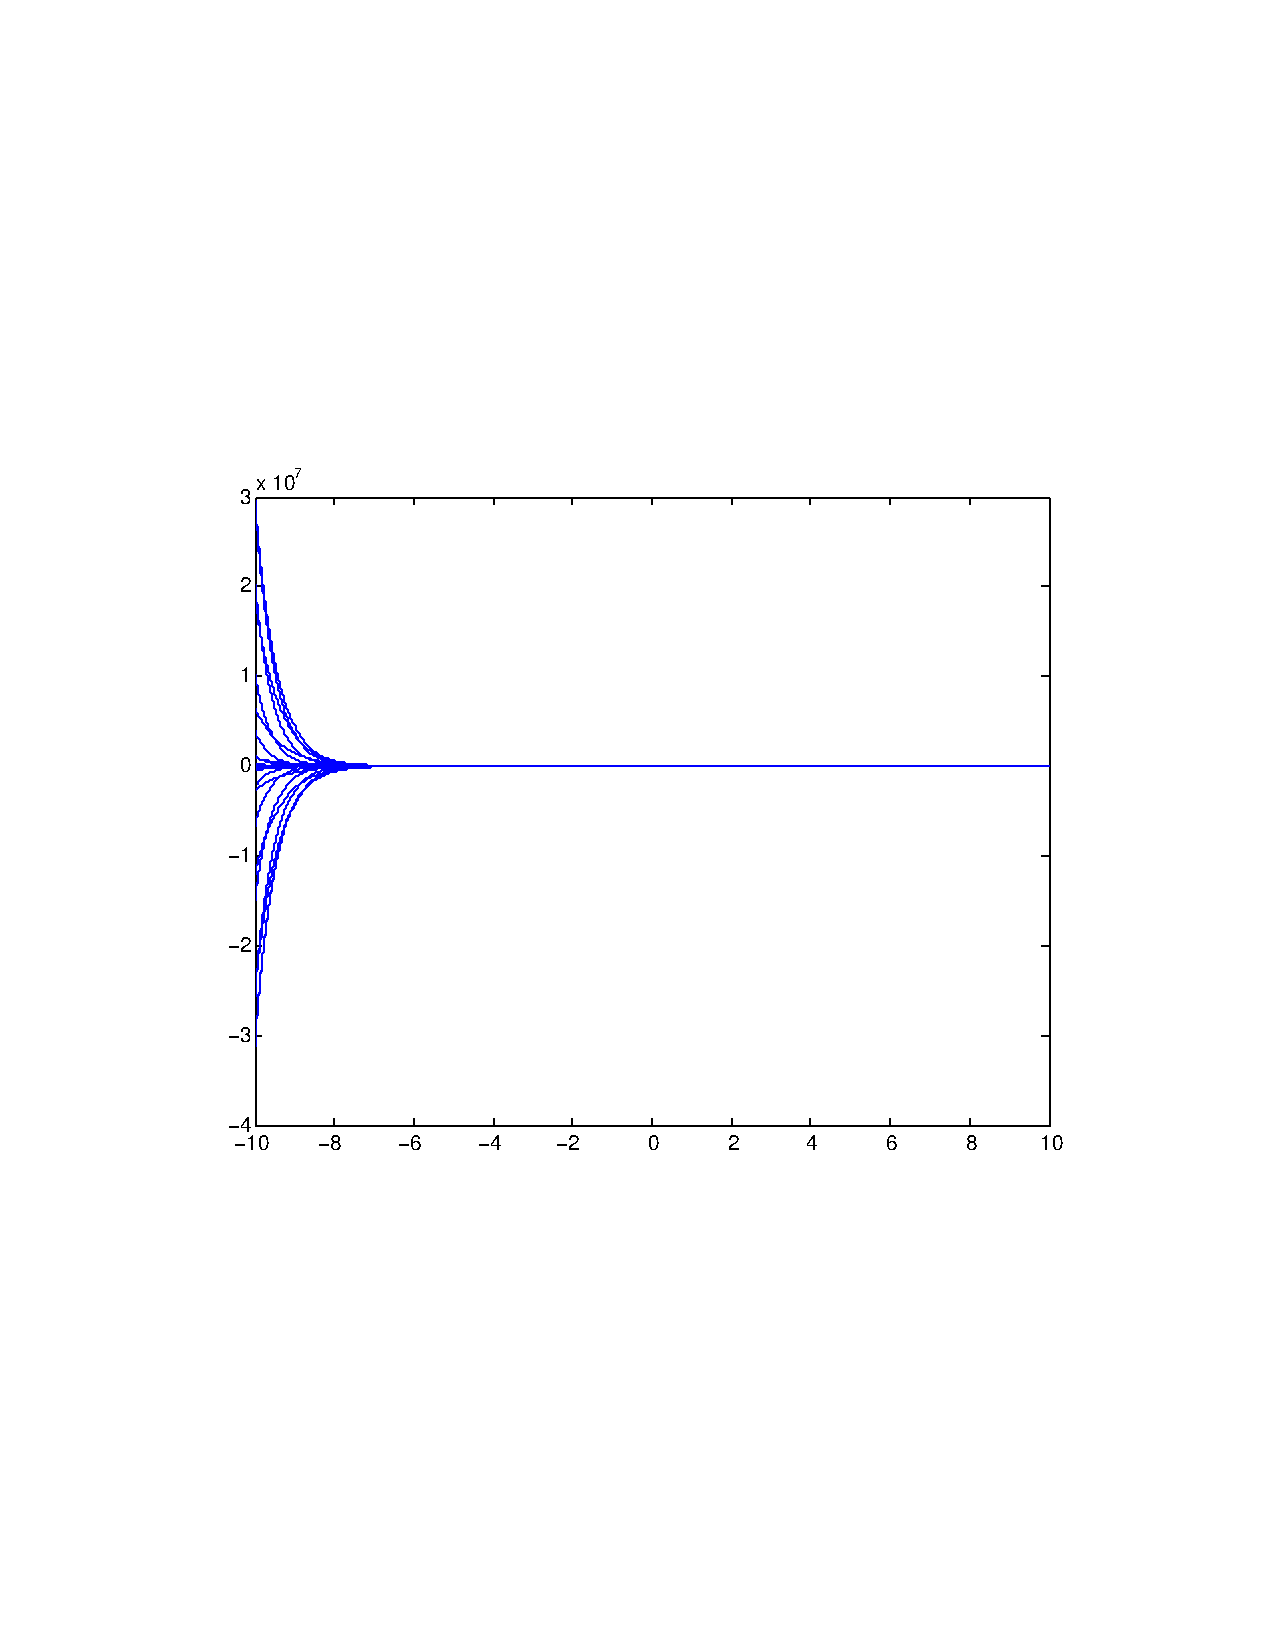
\includegraphics[height=7cm]{figures/calcexp}
\end{center}
\end{frame}

\begin{frame}[fragile]{Auslöschung}
\begin{matlabin}
% Ausloeschung, mit 6 Dezimalstellen
format long g % sorgt fuer lange Ausgabezahlen
x = 0.344152
xwahr = 0.344152*1.0000001 % Fehler
relfx = abs(xwahr-x)/xwahr
y = 0.344135
z = x-y
zwahr = xwahr-y
relfz = abs(z-zwahr)/abs(zwahr) % relativer Fehler von z
\end{matlabin}
\begin{matlab}
x = 0.344152
xwahr = 0.3441520344152
relfx = 9.99999900671778e-08
y = 0.344135
z = 1.69999999999892e-05
zwahr = 1.70344152000124e-05
relfz = 0.00202033352005498
\end{matlab}

\end{frame}



%
% Folie
%
\begin{frame}[fragile]{Komplexe Zahlen}
Komplexe Zahlen $z \in \mathbb{C}$ haben die Form
\[ z = x +iy, \quad x,y \in \mathbb{R} \]
mit $i=\sqrt{-1}$. 
\begin{itemize}
  \item \mcode{i,j}(Matlab) \isage{1j}(Python): vordefinierte Variablen für $\sqrt{-1}$ .
\item \mcode{complex(x,y)}: Erzeugung der komplexen Zahl $x + iy$ aus $x,y \in
  \mathbb{R}$.
\item \mcode{real(z)}: Realteil für $z=x+iy \in \mathbb{C}$ 
\item \mcode{imag(z)}: Imaginärteil für $z=x+iy \in \mathbb{C}$
\end{itemize} 
\end{frame}
\begin{frame}[fragile]{Polarkoordinaten}
\alert{ \[ z \in \mathbb{C}, \quad z=re^{i \varphi}=r(\cos \varphi + i \sin
  \varphi) \]}
\begin{itemize}
\item \mcode{abs(z)} ergibt den Betrag $r$ von $z$.
\item $\varphi$ erhält man durch \mcode{angle(z)}.
\item Matlab: grafische Darst.:  \mcode{compass(z)} ($z=3+3i$). \\
 \centering{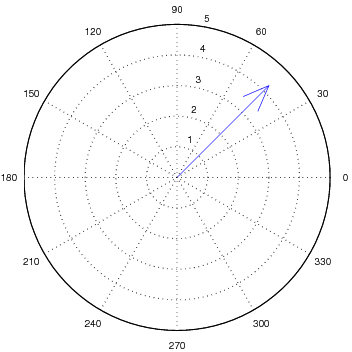
\includegraphics[width=0.3\textwidth]{../figures/kompass}}\\ 
\end{itemize}
\end{frame}

%
% Folie
%
%\begin{frame}[fragile]{Integer}
%\begin{itemize}
%\item In diesen Datentypen werden ganze bzw. nat\"urliche Zahlen gepeichert.  
%\item Zur effizienten Speicherung gibt es die Datentypen \mcode{int8},
%\mcode{uint8}, \mcode{int16}, \mcode{uint16}, \mcode{uint16}, \mcode{int32},
%\mcode{uint32}, \mcode{int64}, \mcode{uint64}. 
%\item In den Datentypen, die mit \mcode{u} beginnen, werden nat\"urliche Zahlen
%gespeichert, sonst ganze Zahlen.
%\item Die abschlie{\ss}ende Zahl gibt den Speicherbedarf an. \mcode{uint8}
%ben\"otigt z.B. $8$-Bit. (Wertebereich $0 \dots 2^8-1$).
%\end{itemize}
%\end{frame}
%
% Folie
%
%\begin{frame}[fragile]{Integer}
%\begin{matlabin}
%a = int8(20); b = int16(20); c = int8(20);
%a*c, a*b
%\end{matlabin}
%\begin{matlab}
%ans =  127
%??? Error using ==> mtimes
%Integers can only be combined with integers
%of the same class, or scalar doubles.
%\end{matlab}
%\begin{matlabin}
%a+0.2
%\end{matlabin}
%\begin{matlab}
%ans =   20
%\end{matlab}
%\begin{matlabin}
%a+0.5
%\end{matlabin}
%\begin{matlab}
%ans =   21
%\end{matlab}
%\begin{matlabin}
%a*1.54
%\end{matlabin}
%\begin{matlab}
%ans =   31
%\end{matlab}
%\end{frame}
%
%
%

\subsection{Container}
%
% Folie
%
\begin{frame}[fragile]{Matlab: Structures}
%(Python: Listen oder Wörterbücher)\\
\alert{Structures:}\\
Strukturen sind eine Möglichkeit verschiedene Objekte in einer
Datenstruktur zu bündeln.\\[1cm]

\alert{Beispiel:} komplexe Zahlen
\begin{matlabin}
komp_Zahl.real=1;
komp_Zahl.imag=1;
komp_Zahl
\end{matlabin}
\begin{matlab}
komp_Zahl = 

    real: 1
    imag: 1
\end{matlab}
\end{frame}
%
% Folie
%
\begin{frame}[fragile]{}
\begin{itemize}
\item Alternativ können Strukturen durch
\begin{matlabin}
struktur = struct('Feld1',<Wert1>,'Feld2',<Wert2>,..)
\end{matlabin}
definiert werden.
\item Ein Feld einer Struktur \mcode{struktur} kann durch 
\begin{matlabin}
struc2 = rmfield( <struktur> ,'Feld')
\end{matlabin}
gel\"oscht werden. 
\end{itemize}
\end{frame}
%
% Folie
%
\begin{frame}[fragile]{Matlab: Cell Arrays}
(Python: Listen)\\
\alert{Cell Arrays:} \\
Cell Arrays sind spezielle Matrizen, deren  Einträge aus unterschiedlichen
Datentypen bestehen können. Erzeugt
werden sie durch geschweifte Klammern.\\
\begin{matlabin}
C = { 1:10, hilb(4);...
       'Hilbert Matrix', pi}
\end{matlabin} 
\begin{matlab}
C = 
       [1x10 double]    [4x4 double]
    'Hilbert Matrix'    [    3.1416]
\end{matlab} 
\end{frame}
%
% Folie
%
\begin{frame}[fragile]{}
\begin{itemize}
\item Zugriff auf Cell-Arrays:\\ 
\begin{columns}[c]
\column{0.45\textwidth}
\begin{matlabin} 
C{2,1}
\end{matlabin}
\begin{matlab}
ans =
Hilbert Matrix
\end{matlab}
\column{0.45\textwidth}
\begin{matlabin}
C{1,2}(2,3)
\end{matlabin}
\begin{matlab}
ans =
    0.2500
\end{matlab}
\end{columns}
\item \mcode{celldisp(C)}: Der Inhalt von $C$ wird dargestellt.
%\item \mcode{struct2cell} bzw. \mcode{num2cell} erzeugt ein Cell Array
%  aus einer Struktur bzw. einer normalen Matrix.
\item \mcode{cellplot(C)} stellt $C$ grafisch dar.
\end{itemize}
\end{frame}

\begin{frame}[fragile]{Python: Wörterbücher (Dictionaries)}
\begin{itemize}
\item Index kann Namen enthalten.
\item Sind gut geeignet für das Speichern großer Datenmengen, da der indizierte Zugriff sehr schnell ist. 
\item der Index ist eindeutig
\item \isage{T = \{\}}: leeres Dictionary
\item Wird ein Index nicht gefunden, gibt es eine Fehlermeldung
\item \isage{T.pop()}: Entnehmen (Löschen und Zurückgeben) von Einträgen 
\item Iterieren:
\begin{pyin}
d = {'a': 1, 'b':1.2, 'c':1j}
for key, val in d.iteritems():
  print key,val        
\end{pyin}
\begin{pyout}
a 1
c 1j
b 1.2
\end{pyout}
\end{itemize}
\end{frame}

\begin{frame}[fragile]{Python: strukturierte array}
  \textbf{Datentypen für Arrays (\isage{dtypes})}
  \begin{itemize}
    \item Types: \isage{int} , \isage{uint} , \isage{float}, \isage{complex}, \isage{string} \ldots
    \item Character Codes : '<typechar><bytes>' : 'i4', 'u4', 'f8', 'c16', 'S25'
    \item typecast: \isage{<object>.astype(<type>)}
  \end{itemize}
Beispiel:
  \begin{pyin}
b = np.array([5, 12345, 'test'],dtype='S4')
  \end{pyin}
\begin{pyout}
array(['5', '1234', 'test'], dtype='|S4')
\end{pyout}
\textbf{Typen definieren}
\begin{pyin}
dt = np.dtype('i4',(2,2)) # 2x2 integer array
\end{pyin}
\textbf{Strukturierte Arrays}
\begin{pyin}
ct = zeros(6, dtype=[('name','S40'),('pop','u4') ])
ct[0]['name'] = 'Auckland'
ct[0]['pop'] = 1418000; ct[0]
\end{pyin}
\begin{pyout}
('Auckland', 1418000L)
\end{pyout}
\end{frame}




\subsection{Chars und Strings}
%
% Folie
%
\begin{frame}[fragile]{Strings }
\emph{Characters (char) - Zeichen}
\begin{itemize}
 \item Darstellung durch Integer
 \item Die Werte zwischen 0 und 128 entsprechen den ASCII Werten (Stichwort Encoding). 
\item 2 Bytes Speicherbedarf $\Rightarrow$ Zahl zwischen 0 und $2^{16}-1$ 
\end{itemize}

\begin{matlabin}
s='d'
\end{matlabin}
\begin{matlab}
s = d
\end{matlab}
\emph{Strings - Vektoren von Zeichen}:
\begin{itemize}
\item Die Zeichen werden wiederum durch die ASCII Werte dargestellt.
\end{itemize}
\begin{matlabin}
s='AB6de*'
\end{matlabin}  
\begin{matlab}
s =
AB6de*
\end{matlab}
%\begin{matlabin}
%s1=double(s)
%\end{matlabin}
%\begin{matlab}
%s1 =  100
%\end{matlab}
%\begin{matlabin}
%s2=char(100)
%\end{matlabin}
%\begin{matlab}
%s2 = d
%\end{matlab}
\end{frame}
%
% Folie
%
%\begin{frame}[fragile]{Strings - Vektor von Zeichen}
%\begin{matlabin}
%sd=double(s)
%\end{matlabin}  
%\begin{matlab}
%sd =
%    65    66    54   100   101    42
%\end{matlab}
%\begin{matlabin}
%s2=char(sd)
%\end{matlabin}  
%\begin{matlab}
%s2 =
%AB6de*
%\end{matlab}
%\end{frame}

%
% Folie
%
\begin{frame}[fragile]{Befehle für Strings}
\begin{itemize}
\item Verbinden von Strings: \mcode{strcat}(Matlab) \isage{+}(Python)  
\begin{matlabin}
strcat('Hello',' world') 
\end{matlabin}
\begin{pyin}
'Hello'+' world'
\end{pyin}
\begin{matlab}
Hello world 
\end{matlab}
\item \mcode{num2str(x,n)}(Matlab) konvertiert $x$ in einen String mit $n$
  signifikanten Stellen. (Default: $n=4$)
\item \isage{str(x)}(Python) konvertiert $x$ in einen String.
%\item \mcode{int2str(x)}(Matlab) rundet $x$ und konvertiert es in einen String.
%\item \isage{int(x)}(Python) rundet $x$ und konvertiert es in einen String.
\item \mcode{strcmp(s,t)}(Matlab) \isage{s==t}(Python) vergleicht die Strings $s$ und $t$. 
\end{itemize}
\end{frame}

\begin{frame}[fragile]{Matlab: Einstieg Standardausgabe}
\begin{matlabin}
fprintf ('Text %<format> und %<format> ... ', x,y,...)
\end{matlabin}
Auszug Formatspezifikation:
\begin{itemize}
\item  \mcode{\%i} : integer
\item \mcode{\%f} : float
\item \mcode{\%s} : strings
\end{itemize}
\emph{Beispiel:}
\begin{matlabin}
fprintf ('Pi mit %i Nachkomma - Stellen : %f \n',6,pi)
\end{matlabin}
\begin{matlab}
Pi mit 6 Nachkomma - Stellen : 3.141593
\end{matlab}
\end{frame}


\begin{frame}[fragile]{Python: Einstieg Standardausgabe}
\begin{pyin}
"Text {<format>} und {<format>} ... ".format(x,y,...)
\end{pyin}
  \isage{<format>}: kann leer bleiben oder eine Reihenfolge enthalten.  Es kann beliebig viele format-Platzhalter geben. (Später Formatspezifikation)
\emph{Beispiel:}
\begin{pyin}
x = 4
y = 6
print ("x ist {0} und y ist {1}".format(x,y))
["x{}".format(k) for k in arange(1,3)]
\end{pyin}
\begin{pyout}
x ist 4 und y ist 6
['x1', 'x2']
\end{pyout}

\end{frame}
         

\end{document}
